
\documentclass[ms.tex]{subfiles}
\begin{document}

\section{Discussion and Conclusions}
\label{sec:conclusions}

% fig 5
\begin{figure*}
\centering
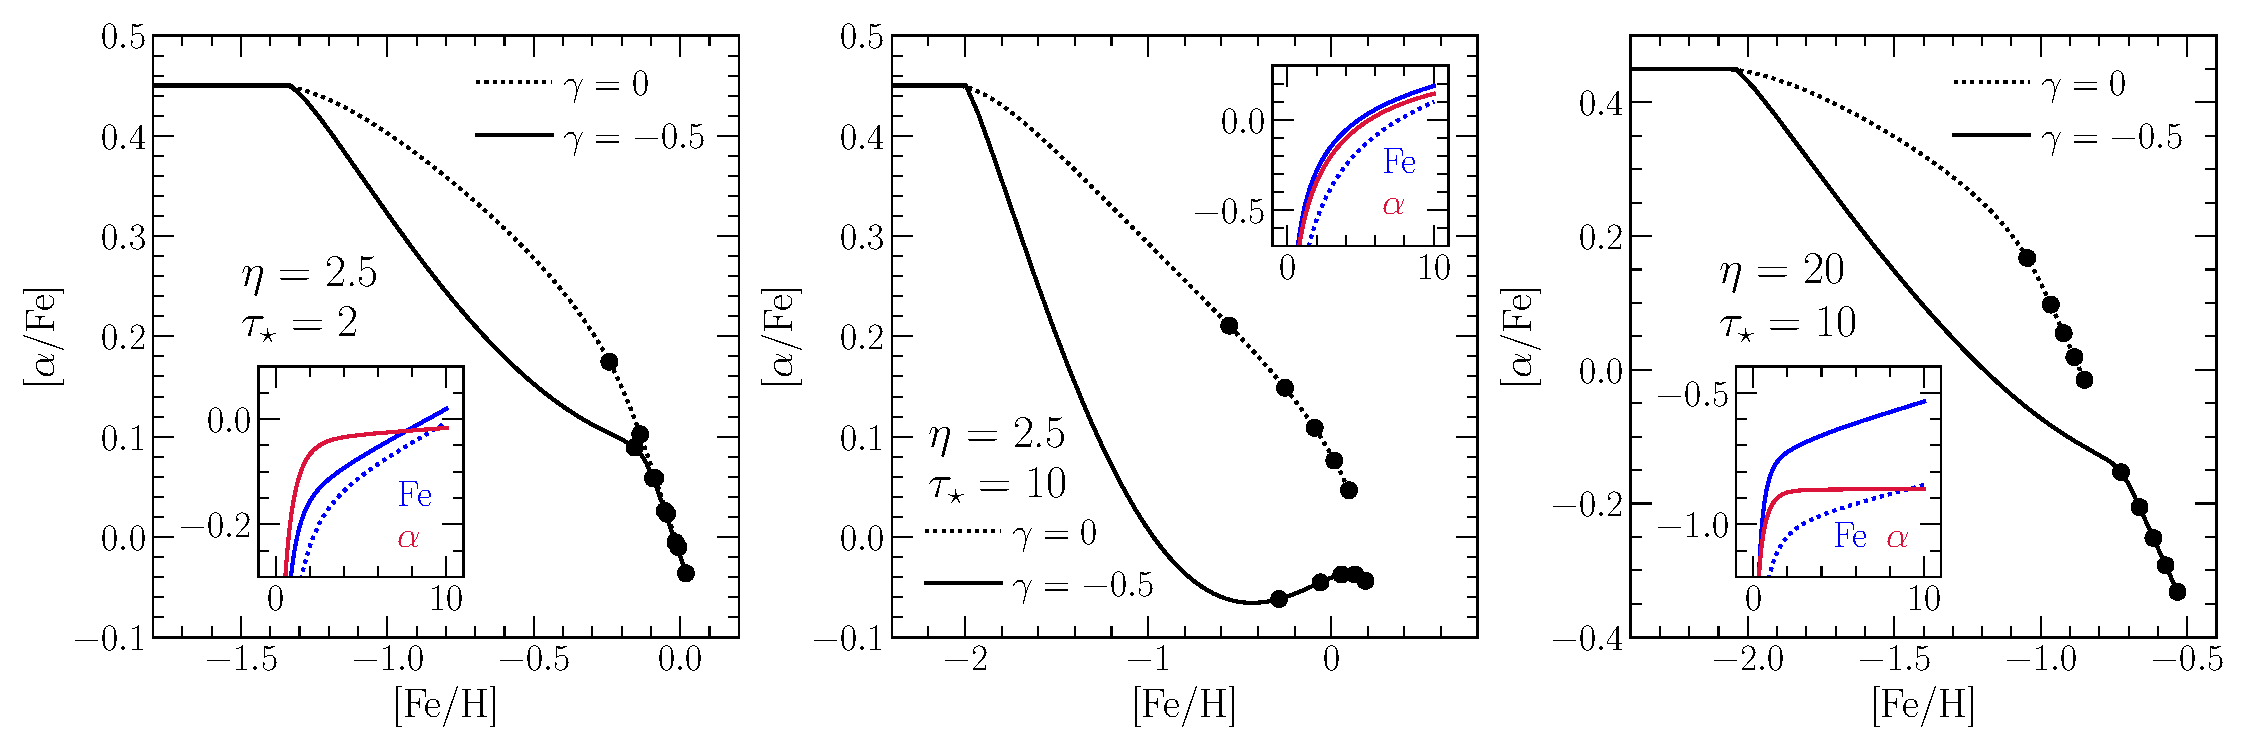
\includegraphics[scale = 0.47]{onezone_application.pdf}
\caption{
A comparison of one-zone galactic chemical evolution models based on
\citet[][for details, see their~\S~2]{Johnson2020} with ($\gamma = -0.5$,
solid) and without ($\gamma = 0$, dotted) metallicity-dependent SN Ia rates.
Tracks denote the O and Fe abundances in the interstellar medium parametrized
as a function of time with points marked at~$T = 2$, 4, 6, 8, and 10 Gyr.
Insets illustrate [O/H] and [Fe/H] as a function of time in Gyr for the
corresponding model.
We note on each panel the choice of the outflow mass-loading factor~$\eta$ and
the star formation efficiency timescale~$\tau_\star$.
}
\label{fig:onezone_app}
\end{figure*}

Building on LOSS~\citep{Li2011},~\citet{Brown2019} and~\citet{Wiseman2021}
found the SN Ia rates rise steeply toward low stellar mass.
The exact slope depends on the adopted SMF, with
$\dot{\text{N}} / \mstar \sim \mstar^{-0.3}$ for~\citet{Baldry2012} and
$\dot{\text{N}} / \mstar \sim \mstar^{-0.5}$ for~\citet{Bell2003}.
To explain this scaling with mass, we use the mean SFHs of galaxies predicted
by the~\um~\citep{Behroozi2019} semi-analytic model of galaxy formation, a
standard~$\tau^{-1}$ DTD~\citep[e.g.,][]{Maoz2012a}, and the empirical MZR as
parametrized by~\citet{Zahid2014} to relate stellar mass to metallicity and
build-in a~$Z^\gamma$ dependence.
Our results depend only on the shape of the MZR and not its absolute
calibration.
While lower mass galaxies have younger stellar populations, we find that this
accounts for only a factor of~$\sim$2 increase in the specific rate between
$\mstar = 10^{7.2}$ and~$10^{10}~\msun$.
We can match the~$\mstar^{-0.3}$ increase if~$\gamma \approx -0.5$,
but~$\gamma \approx -1.5$ is required to explain the steeper
$\dot{\text{N}} / \mstar \sim \mstar^{-0.5}$ scaling.
% We combined the mean SFHs of galaxies as predicted by
% the~\um~\citep{Behroozi2019}semi-analytic model of galaxy formation with the
% empirical MZR as parametrized by~\citet{Zahid2014} to explain the dependence
% of the specific SN Ia rate on stellar mass.
% The young stellar populations of low mass galaxies have high specific SN Ia
% ratesin both ASAS-SN~\citep{Brown2019} and DES~\citep{Wiseman2021}.
% We find that the mean SFHs of galaxies of different stellar masses accounts for
% only a factor of~$\sim$2 increase in the specific SN Ia rate between $10^{10}$
% and~$10^{7.2}~\msun$.
% An additional metallicity dependence of~$Z^\gamma$ where~$\gamma \approx -0.5$
% is required to explain a stellar mass dependence
% of~$\dot{\text{N}}_\text{Ia} / \mstar \sim \mstar^{-0.3}$.
% Normalizing the observed rates by the~\citet{Baldry2012} SMF yields this
% scaling, but the shallower~\citet{Bell2003} predicts
% $\dot{\text{N}}_\text{Ia} / \mstar \sim \mstar^{-0.5}$, which instead requires
% $\gamma \approx -1.5$.
% However, scalings stronger than~$\gamma \lesssim -1$ fail to reproduce
% well-known correlations of [Mg/Fe] and [Fe/H] abundances~\citet{Gandhi2022}.
\par
A scaling of~$\gamma = -0.5$ is in excellent agreement with the dependence of
the close binary fraction measured in APOGEE, which increases from~$\sim$10\%
at~$\sim$$3Z_\odot$ to~$\sim$40\% at~$\sim$$0.1Z_\odot$~\citep{Moe2019}.
This close match suggests that if a scaling of
$\dot{\text{N}}_\text{Ia} / \mstar \sim \mstar^{-0.3}$ is accurate, then the
elevated SN Ia rates in dwarf galaxies can be explained by a combination of
their more extended SFHs and an increased binary fraction compared to their
higher mass counterparts due to differences in metallicity.
While~\citet{Gandhi2022} motivate their investigation from this viewpoint, here
we take this argument one step further and postulate that this accounts for
the~\textit{entire} increase in the specific SN Ia rate because the binary
fraction can naturally account for a factor of~$\sim$3 increase over
the~$\sim$1 decade in metallicity spanned by~$\mstar = 10^{7.2} - 10^{10}
\msun$ galaxies.
The suggestion by~\citet{Kistler2013} that the increased WD mass at low
metallicities drives the effect is likely a subdominant effect.
High mass WDs at low~$Z$ may be an important component if the
steeper~$\sim \mstar^{-0.5}$ scaling inferred with the~\citet{Bell2003} SMF is
correct.
\par
At first glance, an inverse dependence of SN Ia rates on metallicity may seem
at odds with the results in~\citet{Holoien2022} finding that dwarf galaxy
hosts of ASAS-SN SNe Ia tend to be oxygen-rich relative to similar mass
galaxies.
However, SN hosts are likely not a representative sample of the underlying
galaxy population because the steeply declining DTD~\citep[e.g.,][]{Maoz2012a}
means that the intrinsically highest SN Ia rates at any mass should be in
systems which experienced a recent starburst ($\lesssim$1 Gyr ago).
Since oxygen is produced by massive stars with short lifetimes
\citep*[e.g.,][]{Hurley2000, Johnson2019}, these galaxies should also have a
higher-than-average oxygen abundance~\citep[see, e.g.,][]{Johnson2020}.
In other words, SN Ia hosts at fixed mass should be more metal-rich than the
average galaxy.
\par
The calculations we have presented here are simplified in several regards.
We assumed the characteristic SFH predicted by a semi-analytic model of
galaxy formation at all stellar masses.
Our parametrization of the MZR includes no intrinsic scatter, and taking the
\citet{Zahid2014} MZR at face value for use in a power-law scaling implicitly
assumes that all SNe Ia arise from stellar populations near the gas-phase
abundance.
Although in principle galaxies populate distributions of finite width in each
of these quantities, these approximations should be fine for the purposes of
predicting average trends.
\par
Although current surveys lack the depth required to pin down SN rates across
multiple decades of stellar mass at~$z = 1$, the sample sizes necessary to do
so may be available from next-generation facilities.
First and foremost, the Nancy Grace Roman Space Telescope~\citep{Spergel2013,
Spergel2015} will obtain large samples of SNe.
Roman has excellent prospects for discovering all classes of SNe at redshifts
as high as~$z \gtrsim 2$ and beyond~\citep{Petrushevska2016}.
% \par
The difficulty in empirically constraining the specific SN Ia rate at
$z \approx 1$ instead comes from uncertainties in the SMF.
Even at~$z = 0$, these measurements are difficult due to the flux-limited
nature of most surveys and the broad range of luminosities and mass-to-light
ratios spanned by galaxies~\citep[see the discussion in][]{Weigel2016}.
Between~$10^{7.2}$ and~$10^{10}~\msun$, the factors of 2 and 3 predicted by our
calculations with~$\gamma = -0.5$ and $\gamma = 0$ are produced by power-law
indices of~$-0.108$ and~$-0.170$, respectively.
The difference between the two (0.062) is the minimum precision required for
the scaling of the SMF at the low-mass end -- only slightly larger than the
precision achieved by~\citet[][$\pm 0.05$, see their Fig. 13]{Baldry2012}.
This empirical test therefore requires at least their level of precision but
at~$z \approx 1$.
\par
A metallicity dependence of~$Z^{-0.5}$ strongly impacts the evolution of Fe
in one-zone models of galactic chemical evolution.
For a given choice of model parameters, the only regions of chemical space
where~$\gamma = 0$ and~$\gamma = -0.5$ make similar predictions is at
near-Solar abundances and along the high [O/Fe] plateau.
This indicates that best-fit values obtained from fitting one-zone models to
abundances could be significantly impacted by the inclusion of
metallicity-dependent SN Ia rates.
The strongest impact is for dwarf galaxies, where the abundances are low and
the higher yields can shift the endpoint of the evolutionary track by~$\sim$0.5
dex.
% The calculations we have presented here are simplified in several regards.
% First, we have assumed the characteristic SFH predicted by a semi-analytic
% model of galaxy formation at all stellar masses.
% This approximation is reasonable for computing expected mean trends, but in
% principle, the underlying galaxy population should occupy a distribution of
% SFHs.
% \citet{Brown2019} do not find strong evidence that the specific SN Ia rate
% depends on star formation activity at the time of observation, but we do not
% investigate this here because predicted SFHs on a galaxy-by-galaxy basis are
% known to be highly model-dependent~\citep[e.g.][]{Li2020, Hu2022}.
% Second, we have assumed that all galaxies lie perfectly on the MZR, which
% should also be sufficient for computing mean trends.
% However, similar to their SFHs and largely as a consequence thereof, galaxies
% should populate a distribution of metallicities at fixed stellar mass.
% Third, our metallicity scaling of~$Z^\gamma$ where~$Z$ is taken from the
% \citet{Zahid2014} MZR assumes that all SNe Ia in any galaxy arise from stellar
% populations whose metallicities are exactly that of the interstellar
% medium implied by the MZR.
% This approximation is also reasonable because models of galactic chemical
% evolution suggest that galaxies should rapidly approach an equilibrium
% abundance in which the production of new metals is balanced by dilution due to
% accretion of metal-poor gas and losses to star formation and outflows
% \citep{Larson1972, Weinberg2017}.
% Characterizing metal abundances as an equilibrium phenomenon would suggest that
% the young stellar populations which dominate the SN Ia rate (see
% Fig.~\ref{fig:sfh_mzr} and discussion in~\S~\ref{sec:galprops}) should be of
% similar metallicities -- at least on average.
% Although the close binary fraction is known to increase at low abundances
% in APOGEE~\citep{Badenes2018, Moe2019},~\citet{Mazzola2020} find that the
% binary fraction decreases for stars with high [$\alpha$/Fe] ratios at fixed
% [Fe/H], suggesting that the detailed chemical composition may significantly
% impact stellar multiplicity.
% Furthermore, the abundances of metals in stars is a many-dimensional quantity,
% even when grouping them based on their various nucleosynthetic sources
% \citep{Ting2022}.
% However, a theoretical understanding of the metallicity dependence of SN Ia
% rates is a relatively new topic in the literature, and a first-order
% understanding of how the rates scale with the absolute metal abundance in
% statistically average galaxies must be attained before considering how it
% should scale with the detailed chemical composition of the progenitor
% populations.

\end{document}
